\section{Anwendungen}
\subsection{Totale und Bedingte Wahrscheinlichkeit - HIV}
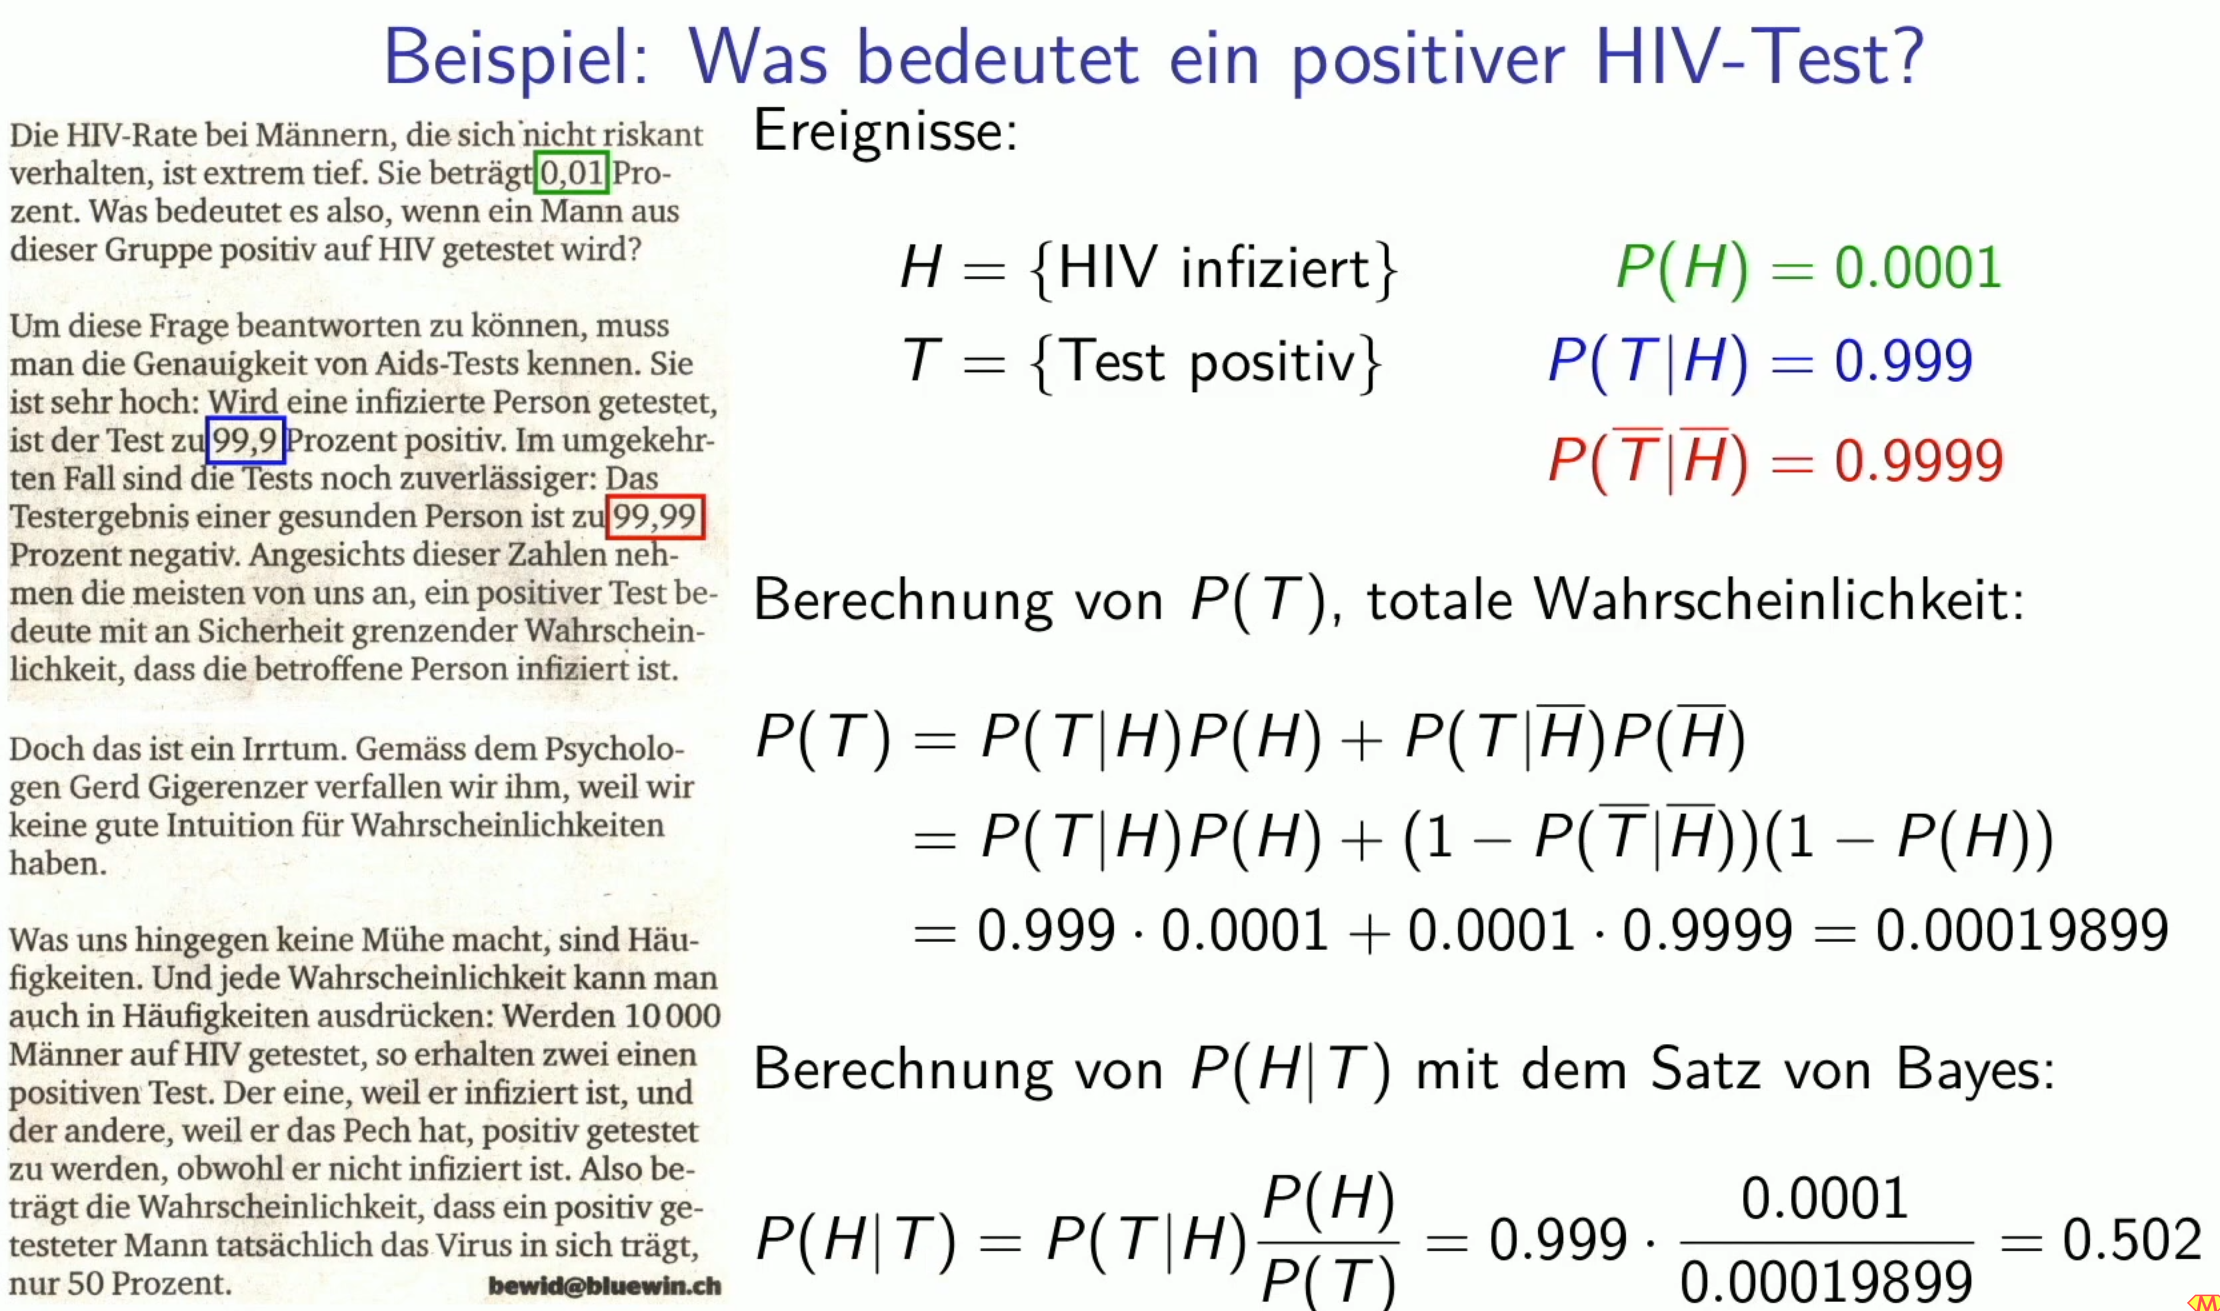
\includegraphics[width=\linewidth]{Images/HIV}

\subsection{Wahrscheinlichkeitsdichte}\label{wdichte}
Gegeb ist Funktion $\varphi(x) = \begin{cases}	a(\cosh 1 - \cosh x) & -1 \le x \le 1\, \\ 0 & \text{sonst}\end{cases}$. Dafür müssen Erwartungswert $\mu$ und Parameter $a$ bestimmt werden.
\begin{center}
	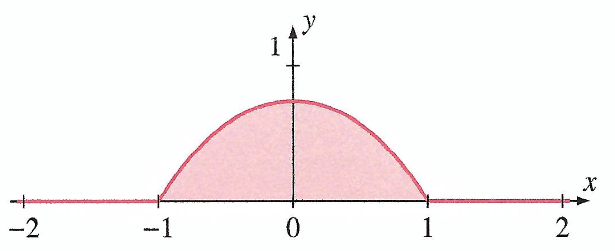
\includegraphics[width=0.6\columnwidth]{Images/wdichte}
\end{center}
\begin{align*}
	\int\limits_{-\infty}^{\infty}\varphi(x)dx &= 1 \xrightarrow{} a\cdot\left[\overbrace{\int\limits_{-1}^{1}\cosh 1dx}^{\circledb{f}} - \overbrace{\int\limits_{-1}^{1}\cosh xdx}^{\circledb{g}}\right] = 1\\
	\circledb{f:} \cosh 1\cdot\int\limits_{-1}^{1}dx &= 2\cdot\cosh(1)\\
	\circledb{g:} \int\limits_{-1}^{1}\cosh xdx &= 2\cdot\sinh(1)\\
	1 &= a\cdot \left(2\cdot \frac{e^1+e^{}-1}{2} - 2\cdot\frac{e^x-e^{-x}}{2}\right) \\
	1 &= a \cdot\frac{2}{e} \\
	a &= \frac{e}{2}
\end{align*}
Da die Funktion \textbf{gerade} ist, ist der Erwarutungswert $\mu = 0$
\subsection{Binomialverteilung Approximation}
Bei einer Umfrage sind $18\%$ der Meinung, die Mondlandung sei eine Verschwörung. Wie Gross ist die Wahrscheinlichkeit, dass in einer Stichprobe von 100 Menschen mehr als 20 finden lassen, die die Mondlandung für eine Verschwörung halten? Im Vergleich sind Flat Earther selten mit $1.28\%$
\subsubsection{Normalverteilung}\label{approx_normal}
$X$ ist die Anzahl Mondlandungsverweigerer. $X$ ist Binomialverteilt mit $p=0.18$ und $n=100$. Daraus lässt sich $\mu=np = 18$ und $\sigma = \sqrt{np(1-p)} = 3.84187$ berechnen.
\begin{align*}
	P(X \gt 20) &= 1 - P(X \le 20) \\
	P(X \le 20) &= P\left(\frac{X - \mu}{\sigma} \le \frac{20 + 0.5 - \mu}{\sigma}\right) = \Phi(0.6507) = 0.7424\\
	P(X \gt 20) &\approxeq 1 - 0.7424 = 0.2576
\end{align*}

\subsubsection{Poissionverteilung}\label{approx_poission}
$X$ ist die Anzahl Flath Earthler. Die erwartet Anzahl ist daher $\lambda = np = 1.28$
\begin{align*}
	P(X \gt 2) &= 1 - P(X \le 2) = 1 - P(X =0) - P(X=1) - P(X=2) \\
	&= 1-P_\lambda(0) -P_\lambda(1)-P_\lambda(2)\\
	&= 1 - e^{-\lambda}\left(1 + \lambda + \frac{\lambda^2}{2}\right)\\
	&= 1 - 0.86169 = 0.138307
\end{align*}

\subsection{Schätzen}\label{konf_intervall}
400 $1k\Omega$ Widerstände wurden ausgemessen. $\frac{1}{4} = 25\%$ hatten einen Wert von über $1000
72\Omega$, $10\%$ nicht mehr als $997.9\Omega$. Wie gross ist der mittlere Widerstand und Standardabweichung dieser Reihe? \textit{Annahmem dass Widerstände normalverteilt sind.}
\begin{align*}
	P(X \le 1000.72) &= 1 - 0.25 = 0.75 \\
	P(X \le 997.9) &= 0.1
\end{align*}
\begin{center}
	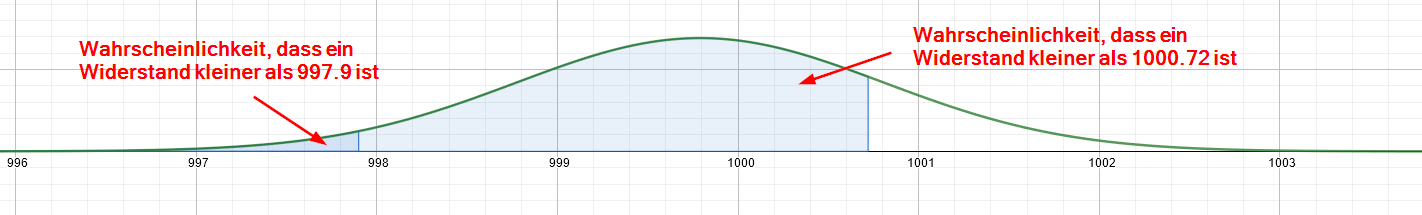
\includegraphics[width=\columnwidth]{Images/schätzen}
\end{center}
Durch standardisierung und der Quantilentabelle aus Kapitel \ref{quantilentabelle} liest man heraus:
\begin{align*}
    P\left(\frac{X - \mu}{\sigma} \le \frac{1000.72 - \mu}{\sigma}\right) &= 0.75 & \xRightarrow[]{}	F(x_+) &= 0.6745 \\
	P\left(\frac{X - \mu}{\sigma} \le \frac{997.9 - \mu}{\sigma}\right) &= 0.10 & \xRightarrow[]{}	F(x_-) &= -1.2816
\end{align*}
Was ein Gleichungssystem für $\mu$ und $\sigma$ ergibt. Somit sind $\mu=999.79$ und $\sigma = 1.44\Omega$
\begin{align*}
	1000.72 - \mu = 0.6745\sigma \\
	997.9 - \mu = -1.2816\sigma
\end{align*}

\subsection{Linear Regression}\label{covarianz_eg}\label{regression}
Eine Regression bewerten. Die Geradenkoeffizienten $ a= 0.6278, b = 7.385$ wurden mit LeastSquare gefunden.
\begin{center}
	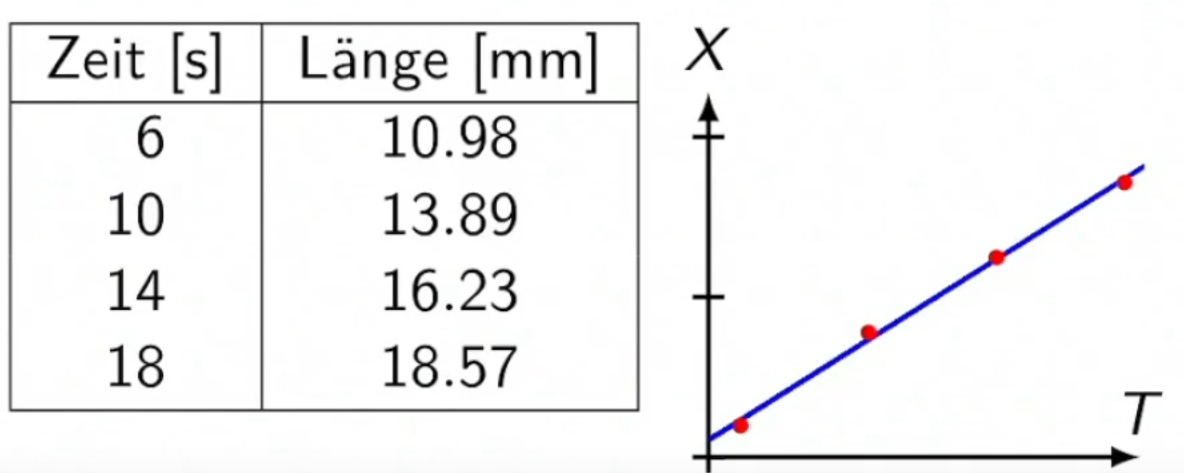
\includegraphics[width=0.5\columnwidth]{Images/regression}
\end{center}

\begin{center}
	\begin{tabular}{l|rr|rr|r}
		$j$ & $t_j$ & $t^2_j$ & $x_i$ & $x_i^2$ & $t_jx_j$ \\ \toprule
		1 & 6 & 36 & 10.98 & 120.6 & 65.88 \\  \midrule
		2 & 10 & 100 & 13.89 & 192.9 & 138.9 \\  \midrule
		3 & 14 & 196 & 16.23 & 263.4 & 227.2\\  \midrule
		4 & 18 & 324 & 18.57 & 344.8 & 334.3 \\  \bottomrule
		$\sum$  & 48 & 656 &  59.67 & 921.74 & 766.26\
	\end{tabular}
\end{center}

\noindent Daraus lassen sich folgende Werte bestimmen:
\begin{align*}
	E(t) &= 12 \qquad E(t^2) = 164  \\
	E(x) &= 14.91 \qquad E(x)^2 = 230.44  \\
	\cov(T, X) &= E(tx) - E(x)E(t) = 191.56 - (14.91 \cdot 12) = 12.56 \\
	\var(t) &= E(t^2) - E(t)^2 = 164 - 144 = 20 \\
	\var(x) &= E(x^2) - E(x)^2 = 230.4 - 222.3 = 8.129 \\
	r^2 &= \frac{\cov(t, x)^2}{\var(t)\var(x)} = \frac{12.56^2}{20\cdot 8.129} = 0.9695
\end{align*}

\noindent Der Wert liegt nahe bei $1$, daher eine recht gute Regression.

\subsection{Hypergeometrische Verteilung}
In einer Kiste mit 20 Äpfeln sind 5 wurmstichig. Wie gross ist die Wahrscheinlichkeit, in einer Stichprobe von 8 Äpfeln 2 wurmstichige zu funden? $N= 20, M = 5, n = 8, m = 2$
\[
P(X= 2) = \frac{\begin{pmatrix} 5 \\ 2 \end{pmatrix}\begin{pmatrix} 15 \\ 6 \end{pmatrix}}{\begin{pmatrix} 20 \\ 8 \end{pmatrix}} = 0.3973
\]


\subsection{Testen einer Verteilung}
\subsubsection{$\chi^2$-Test}\label{tictac}
\textbf{Nullhypothese} $H_0$: Alle Farben sind im TicTac gleich wahrscheinlich, d.h. $p_i = \frac{1}{4}$.\\
Die \textbf{Parameter} sind $4$ Farben, daraus ergeben sich $k= 4 -1 = 3$ Freiheitsgrade. $\alpha = 0.05$ wird in diesem Fall angenommen. Aus der $\chi^2$Tabelle ergibt den Kritischen $D_\text{krit} = 7.815$
\begin{center}
	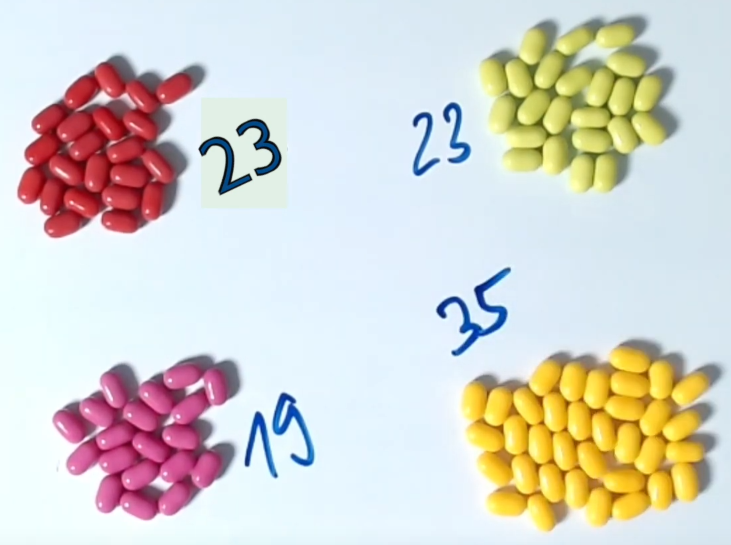
\includegraphics[width=0.8\columnwidth]{Images/tictac}
\end{center}

Damit lässt sich die Diskrepanz berechnen:\\
\begin{center}
	\begin{tabular}{l|rrrrr|}
	Farben $i$ & $p_i$ & $n_i$ & $np_i$ & $n_i - np_i$ & $\frac{(n_i - np_i)^2}{np_i}$ \\ \toprule
	rot & $0.25$ & $23$ & $25$ & $-2$ & $\frac{4}{25}$ \\  \midrule
	pink & $0.25$ & $19$ & $25$ & $-6$ & $\frac{36}{25}$ \\ \midrule
	gelb & $0.25$ & $35$ & $25$ & $10$ & $\frac{100}{25}$ \\ \midrule
	grün & $0.25$ & $23$ & $25$ & $-2$ & $\frac{4}{25}$ \\ \midrule
	& & $n=100$ & & & $D =5.76$ \\ \bottomrule
\end{tabular}
\end{center}

\noindent
$n_i$ Anzahlen, \\
$np_i$ Erwartete Anzahl,  \\
$n_i - np_i$: Abweichungen, \\
$(n_i - np_i)^2/np_i$: Diskrepanz

Da $D < D_{krit}$ ist, gibt es keinen Grund an der Nullhypothese zu zweifeln.

\subsubsection{Kolmogorov-Smirnof Test}\label{Kolmogorov}
Generiert ein Zufallsgenerator im Intervall $[0, 1]$ mit $\alpha=0.01$ eine gleichverteilte Zufallszahl $x_j$? Damit ist in diesem Beispiel $F(x) = x$ (Lineare Verteilung) und $n$ die Anzahl Werte und $j$ der entsprechender sortierte Eintrag ist.
\begin{center}
	\begin{tabular}{l|r|r|r}
		$j$ & $x_j$ & $\frac{i}{n}-F(x_j)$ & $F(x_j) - \frac{i-1}{n}$ \\ \toprule
		1 & 0.00040 & 0.110 & 0.0004  \\  \midrule
		2& 0.00398 & 0.218 & -0.1071 \\  \midrule
		$\vdots$ & $\vdots$& &  \\  \midrule
		i & 0.43987 & 0.560 &-0.4490 \\ \bottomrule
		& & $\max_1(\dots)$ & $\max_2(\dots)$
	\end{tabular}
\end{center}

Damit ist $\max_1 = 0.61222$ und  $\max_1 = 0.00040$ damit lassen sich die $K$ Werte bestimmen:

\[
K_n^+ = \sqrt{n}\cdot \max_1 = 1.83666 \qquad K_n^- = \sqrt{n}\cdot \max_2 = 0.00120
\]

Weil $K_n^+ > K_\text{krit}$ muss die Hypothese verworfen werden, dass die Zufallszahlen gleichverteilt seien.


\subsection{Fehler von Multi-Sensor-System}
\begin{center}
	\begin{tabular}{l|r|r|r}
		& Messbereich & Std.abweichung $\sigma$ & Grundfreq. \\ \toprule
		Sensor 1 & $\pm37g$ & $24mg \rightarrow 0.024$ & $400$Hz  \\  \midrule
		Sensor 2 & $\pm19g$ & $22mg \rightarrow 0.022$ & $1600$Hz \\  \midrule
	\end{tabular}
\end{center}
Wieviel Prozent kann man den Fehler, gemessen mit der Standardabweichung, maximal korrigieren, wenn man beide Messwerte geeignet mittelt?

Die beiden Sensoren $X_1$ und $X_2$ können mit einer Normalverteilung mit gleichem $\mu$ aber verschiedenen Varienzen gemittelt werden. Ziel ist es die $\var(X)$ zu minimieren. 
\begin{align*}
	X &= tX_1 + (1-t)X_2 \\
	\var(X) &= t^2\var(X_1) + (1-t)^2\var(X_2)
\end{align*}
Das Minimum finden durch Nullsetzten der Ableitung
\begin{align*}
	0 = \frac{d}{dt}\var(X) &= 2t\var(X_1) - 2(1-t)\var(X_2) \\
	\rightarrow  \qquad t &= \frac{\sigma_2^2}{\sigma_1^2 + \sigma_2^2} \\
	 1-t &= \frac{\sigma_1^2}{\sigma_1^2 + \sigma_2^2}
\end{align*}
Ein erste Formel einsetzen
\begin{align*}
	\var(X) &= \left(\frac{\sigma_2^2}{\sigma_1^2 + \sigma_2^2}\right)^2\sigma_1^2 + \left(\frac{\sigma_1^2}{\sigma_1^2 + \sigma_2^2}\right)^2\sigma_2^2 \\
	&= \frac{\sigma_1^2\sigma_2^2}{\sigma_1^2+\sigma_2^2}
\end{align*}
und anschliessend $\sigma$ berechnen
\[
\sigma = \sqrt{\var(X)} = \sqrt{\frac{\sigma_1^2\sigma_2^2}{\sigma_1^2+\sigma_2^2}} = \sqrt{\frac{0.022^2\cdot 0.024^2}{0.022^2 + 0.024^2}} = 0.016
\]  
Man kann also den Fehler von $0.022g$ auf $0.016g$ reduzieren, eine Reduktion um $27\%$.

\subsection{Kalman-Filter}\label{kalman}
Die Messgenauigkeit ist $\pm0.1^\circ C$ mit einer Tagsmitteltemperatur von $\pm10^\circ C$. Der Treibhauseffekt von $CO_2$ kann durch die Grösse $p$ beschrieben werden. In einem Zeitintervall $\Delta t$ nimmt die Temperatur
um $p \cdot \Delta t$ zu. $p=0$ bedeutet, dass sich die Temperatur nicht verändert. $p$ kann nicht direkt gemessen werden, daher soll ein Kalman-Filter implementiert werden, welche $p$ aus dem Temperaturmessungen herausfiltert.

Die Systemvariablen sind $T$ und $p$
\[
x_{k+1} = \begin{pmatrix}T_{k+1} \\ p_{k+1} \end{pmatrix} = \begin{pmatrix}T_{k} + p_{k}\Delta t \\ p_k \end{pmatrix} = \underbrace{\begin{pmatrix}1 & \Delta t \\ 0 & 1 \end{pmatrix}}_{\varphi}\begin{pmatrix}T_k \\ p_k \end{pmatrix}
\]
Da nur Temepratur gemessen wird, gilt $H = \begin{pmatrix} 1 & 0 \end{pmatrix}$. Bekannt ist ausserdem die Messgenauigkeit von $0.1K$, welche $R = \begin{pmatrix}0.01K^2\end{pmatrix}$ ergibt. Die Systemfehlerkovarianzmatrix muss folgende Form haben:
\[
Q = \begin{pmatrix}\sigma_T^2 & 0 \\ 0 & \sigma_p^2 \end{pmatrix}
\]
Für $\sigma_T^2$ könnten wir schätzen, dass wir in unserem Modell die Wetterentwicklung nicht modelliert haben, die Temperaturschwankungen müssen also im Systemfehler untergebracht werden. Damit ist $\sigma_T = 10K$. Leider sind keine Informationen über $\sigma_p$ bekannt.